\Chapter{A fejlesztőkörnyezet megvalósítása}

\graphicspath{{./kepek/}}

\Section{Minimális program fájlok kezeléséhez, szerkesztéséhez}

A szoftver megvalósítását egy olyan minimális életképes program elkészítésével kezdjük,
amely meg tud nyitni egyszerre egy fájlt, annak tartalmát megfelelően megjeleníti,
hogy ha az egy Rust forráskód-fájl. Képes a fájlt az eredeti helyén szerkeszteni, vagy egy másik megadott fájlba menteni.

\begin{figure}[h!]
    \centering
    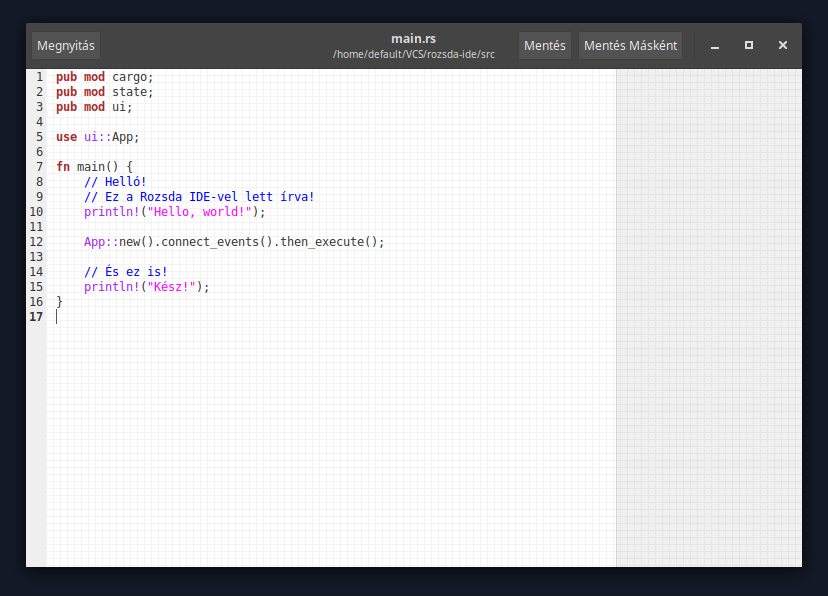
\includegraphics[width=0.8\textwidth]{program-mvp}
    \caption{A kódszerkesztő program a \textit{Hello, World!} alkalmazás kódjával}
	\label{fig:program-mvp}
\end{figure}

A programnak ez a része Michael Murphy \textit{Simple Common Mark Editor} projektjén alapul \cite{gtk_tutorial}.
Murphy programja Markdown formátumú fájlokat kezel, illetve azokat HTML formátumra lefordítja,
és megjeleníti a felhasználónak.
A leglényegesebb változtatások ezen a programon a Markdown nyelv lecserélése jelentette a Rust nyelvre.
További feladat volt még a projekt frissítése egyrészt a Rust 2018-as verziójára, illetve a függőségek frissítése a legújabb verziókra.

A projekt a szokásos módon egy \texttt{cargo new} parancs kiadásával lehetett kezdeni.

% TODO:
% - Megnyitás, mentés
% - ActiveMetadata
% - FileChooserDialog
% - események csatlakoztatása App-ban
% - Main

% TODO: Részletesen be kell mutatni a tervezést és az implementációt!

% Lehet hozzá jó sok ábra. Az implementációnál itt szerepelhetnek kódrészletek.